\section{Verificatie}\label{sec:tests}

%inleiding over welke testen we gaan uitvoeren en waarom. Over hoe de testen zijn opgesteld en wat het doel is van de totaliteit testen.
In dit hoofdstuk worden enkele tests uitgevoerd om het functioneren van het netwerk te evalueren. Hieruit kan worden afgeleid wat de optimale afstanden zijn en welke betrouwbaarheid haalbaar is.

\subsection{Enkele communicatie Test}
% uitleg wat de test is met doel
Deze test evalueert de communicatie tussen twee nodes. Het doel is om te beoordelen hoe betrouwbaar de verbinding is en over welke afstand de communicatie nog steeds betrouwbaar is. Ook zal het vermogen van de chip worden verhoogd. Er is echter niet genoeg ruimte om op vol vermogen te testen, waardoor is gekozen voor de twee laagste vermogens. De test begint door eerst 100 berichten naar de andere node te verzenden op een afstand van 10 cm en te kijken hoeveel van de berichten aankomen bij de andere node. De betrouwbaarheid wordt bepaald op basis van het aantal ontvangen berichten van de 100 verzonden berichten. Daarnaast worden ook de vertrouwensniveaus vastgelegd die het systeem zelf meet. Hiervan wordt een gemiddelde genomen van de tijd tussen het eerste en het laatste bericht. Dit wordt gedaan om de gegevens met elkaar te vergelijken en conclusies te trekken.

% Testopstelling
In afbeelding \ref{fig:TestCom} is de testopstelling weergegeven. Hierop is te zien dat twee XMega's nodig zijn met een NRF-chip. Deze moeten worden geplaatst zoals aangegeven in de testopstelling en na elke test wordt de afstand vergroot volgens de tabel waarin alle testresultaten worden vastgelegd. Bij deze test zal er niets tussen de verbinding zitten.

\begin{figure}[h]
    \centering
    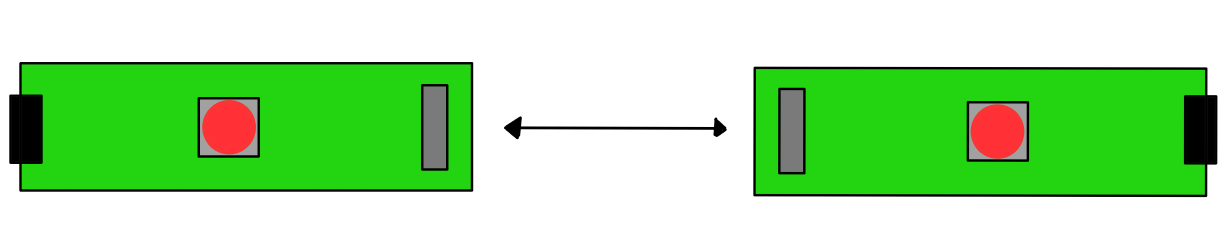
\includegraphics[scale = 0.3]{img/test1.png}
    \caption{Test opstelling.}
    \label{fig:TestCom}
\end{figure}

\vspace{0.5cm}
% Resultaten test

\begin{figure}[ht]
    \centering
    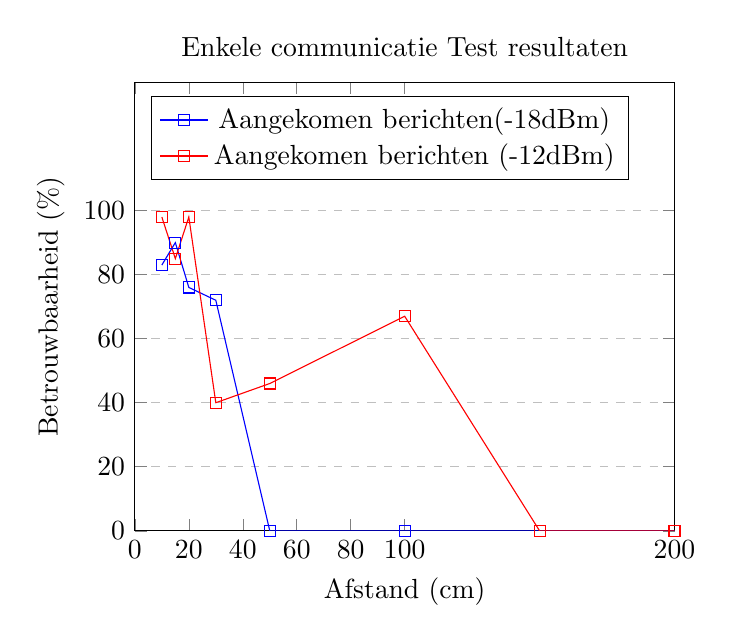
\begin{tikzpicture}
    \begin{axis}[
        title={Enkele communicatie Test resultaten},
        xlabel={Afstand (cm)},
        ylabel={Betrouwbaarheid (\%)},
        xmin=0, xmax=200,
        ymin=0, ymax=140,
        xtick={0,20,40,60,80,100,200},
        ytick={0,20,40,60,80,100},
        legend pos=north west,
        ymajorgrids=true,
        grid style=dashed,
    ]

    \addplot[
        color=blue,
        mark=square,
        ]
        coordinates {
        (10,83)(15,90)(20,76)(30,72)(50,0)(100,0)(150,0)(200,0)
        };
        \addlegendentry{Aangekomen berichten(-18dBm)}

    \addplot[
        color=red,
        mark=square,
        ]
        coordinates {
        (10,98)(15,85)(20,98)(30,40)(50,46)(100,67)(150,0)(200,0)
        };
        \addlegendentry{Aangekomen berichten (-12dBm)}
        
    \end{axis}
    \end{tikzpicture}
\end{figure}

\newpage
\subsection{Hop Test}
% uitleg wat de test is met doel
Deze test is vergelijkbaar met de vorige test, maar maakt gebruik van één extra node tussen de twee versturende en ontvangende nodes. Het doel van deze test is om te onderzoeken hoe betrouwbaar de communicatie via hops is. Ook kan worden gekeken tot welke maximale afstand de hops nog steeds functioneren.

% Testopstelling
Voor deze test zijn drie nodes nodig. In \autoref{fig:Testhop} is te zien hoe de nodes moeten worden geplaatst: één die ontvangt, één die verstuurt en één die wordt gebruikt als hop. Deze test wordt slechts één keer uitgevoerd omdat de afstand al is bepaald in de vorige test. Zodra de berichten aankomen, is de test voltooid.
\begin{figure}[h]
    \centering
    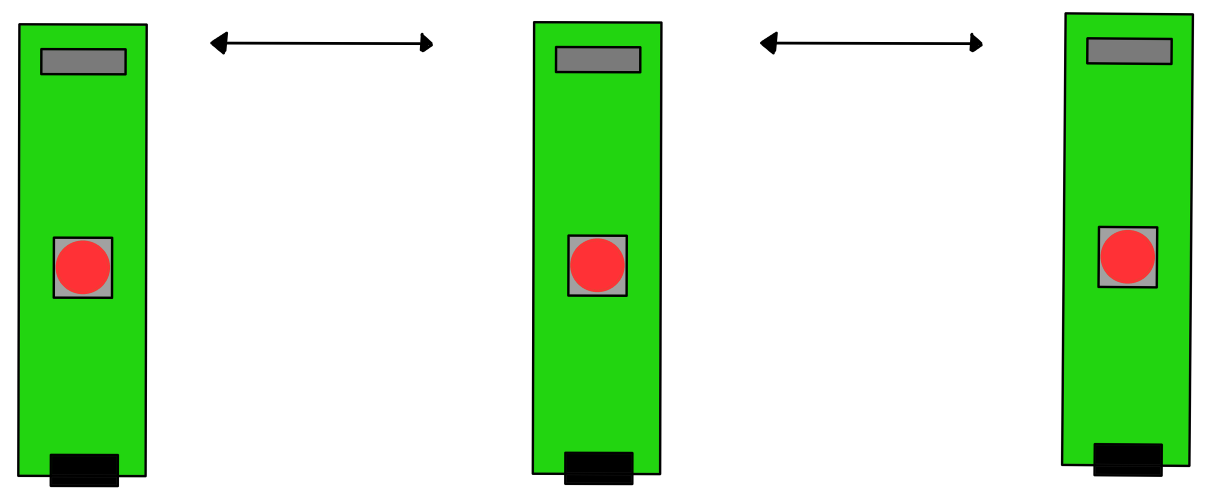
\includegraphics[scale = 0.4]{img/test2.png}
    \caption{Test opstelling 2}
    \label{fig:Testhop}
\end{figure}

% Resultaten test
\begin{figure}
    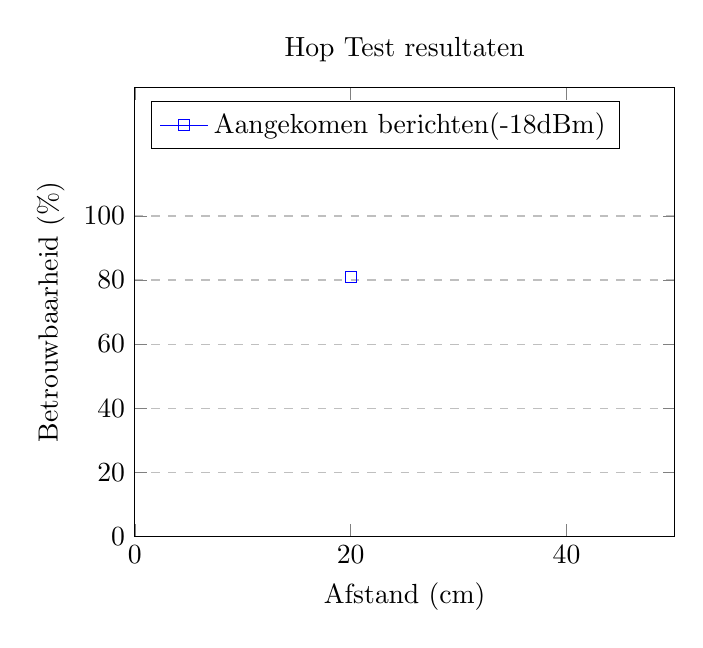
\begin{tikzpicture}
    \centering
    \begin{axis}[
        title={Hop Test resultaten},
        xlabel={Afstand (cm)},
        ylabel={Betrouwbaarheid (\%)},
        xmin=0, xmax=50,
        ymin=0, ymax=140,
        xtick={0,20,40},
        ytick={0,20,40,60,80,100},
        legend pos=north west,
        ymajorgrids=true,
        grid style=dashed,
    ]

    \addplot[
        color=blue,
        mark=square,
        ]
        coordinates {
        (20,81)
        };
        \addlegendentry{Aangekomen berichten(-18dBm)}
    \end{axis}
    \end{tikzpicture}
\end{figure}


% \newpage
% \subsection{Totale communicatie Test}
% % uitleg wat de test is met doel
% Deze test is een samenvoeging van de vorige twee tests. In deze test wordt gekeken naar de communicatie tussen meerdere nodes. Elke node zal 100 berichten versturen naar een zelfgekozen node, waarbij de keuze bestaat uit een node met één of meerdere hops en een directe node. De afstand blijft statisch in deze test. Het doel van deze test is om te beoordelen of de communicatie met meerdere nodes succesvol is en of elke node vergelijkbare resultaten vertoont.

% % Testopstelling
% Aangezien het onderwerp van dit verslag betrekking heeft op vijf sensoren met een basisstation, zullen voor deze test zes afzonderlijke nodes worden gebruikt. In onderstaande afbeelding \ref{fig:TestTotCom} is te zien hoe de XMega's moeten worden opgesteld. De afstand is gebaseerd op de grootst mogelijke afstand waarbij de betrouwbaarheid nog boven de 90\% ligt, zoals vastgesteld in de eerdere enkele communicatietest.

% \begin{figure}[h]
%     \centering
%     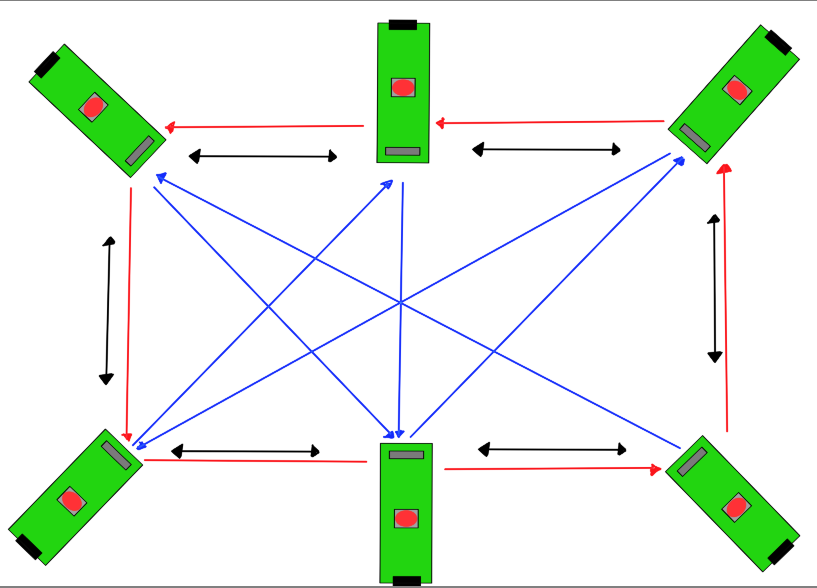
\includegraphics[scale = 0.5]{img/test3.png}
%     \caption{Test opstelling 3}
%     \label{fig:TestTotCom}
% \end{figure}

% \begin{figure}[h]
%     \centering
%     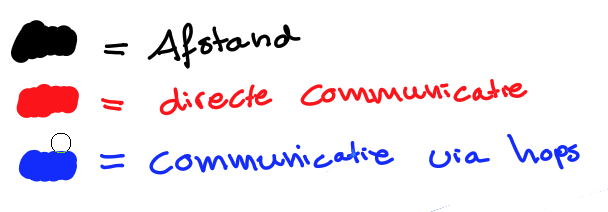
\includegraphics[scale = 0.3]{img/legenda_test3.png}
%     \caption{Legenda Test opstelling 3}
%     \label{fig:TestTotComLeg}
% \end{figure}

% % Resultaten test
% In tabel \ref{Test:TotCom} zijn de testresultaten te zien, zowel die van de directe buur als die van de indirecte buur.
% \begin{table}[h]
%     \centering
%     \begin{tabular}{|c||c|c|c|c|c|}
%         \hline
%         \textbf{Test}    & \textbf{Node}  & \textbf{Directe buur}   & \textbf{Aangekomen berichten}  & \textbf{Trust}     & \textbf{Betrouwbaarheid}   \\\hline\hline
%         Test 1  &       &                &                       &           &                   \\\hline
%         Test 2  &       &                &                       &           &                   \\\hline
%         Test 3  &       &                &                       &           &                   \\\hline
%         Test 4  &       &                &                       &           &                   \\\hline
%         Test 5  &       &                &                       &           &                   \\\hline
%         Test 6  &       &                &                       &           &                   \\\hline
%     \end{tabular}
%     \caption{Testresultaten Totale communicatie Test (Directe buur).}
%     \label{Test:TotCom}
% \end{table}

% \begin{table}[h]
%     \centering
%     \begin{tabular}{|c||c|c|c|c|c|c|}
%         \hline
%         \textbf{Test}    & \textbf{Node}  & \textbf{Indirecte buur}   & \textbf{Aantal hops} & \textbf{Aangekomen berichten}  & \textbf{Trust}     & \textbf{Betrouwbaarheid}   \\\hline\hline
%         Test 1  &       &                &           &            &           &                   \\\hline
%         Test 2  &       &                &           &            &           &                   \\\hline
%         Test 3  &       &                &           &            &           &                   \\\hline
%         Test 4  &       &                &           &            &           &                   \\\hline
%         Test 5  &       &                &           &            &           &                   \\\hline
%         Test 6  &       &                &           &            &           &                   \\\hline
%     \end{tabular}
%     \caption{Testresultaten Totale communicatie Test (Indirecte buur).}
%     \label{Test:TotCom}
% \end{table}

% \newpage
% \subsection{Encryptie Test}
% % uitleg wat de test is met doel
% Deze test controleert of de encryptie correct is geïmplementeerd. Dit wordt gedaan door twee nodes te nemen en bij één node de encryptie uit te schakelen. Vervolgens wordt gekeken naar wat binnenkomt en wordt dit bericht handmatig ontcijferd. Nadat dit is gedaan, wordt de encryptie weer ingeschakeld om te controleren of dit overeenkomt met wat is verzonden. Het doel van deze test is om te kijken of de encryptie naar behoren werkt.

% % Testopstelling
% De opstelling is hetzelfde als die van de enkele communicatietest. Het enige verschil is de encryptie die bij één node is ingeschakeld en bij de andere uitgeschakeld.\begin{figure}[h]
%     \centering
%     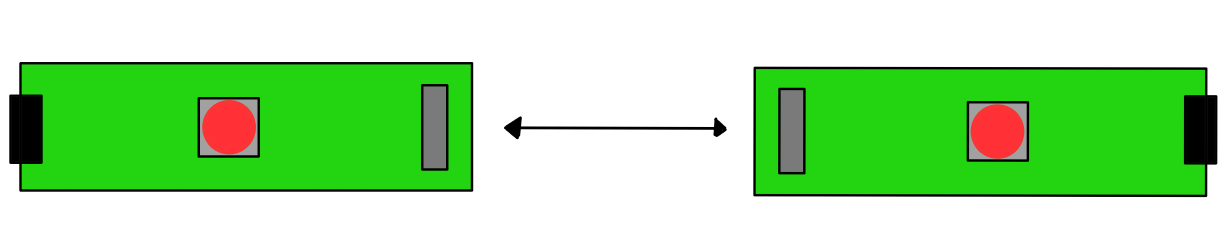
\includegraphics[scale = 0.3]{img/test1.png}
%     \caption{Test opstelling}
%     \label{fig:TestEn}
% \end{figure}
% % Resultaten test
% \begin{table}[h]
%     \centering
%     \begin{tabular}{|c||c|c|c|c|c|c|}
%         \hline
%         Test    & Verzonden bericht      & Key 1 & Key 2 & Ontvangen bericht & Zelf Decrypted bericht & Decrypted bericht \\\hline
%         Test 1  & Hallo                  &       &       &                   &                        &                   \\\hline
%         Test 2  & Poezen zijn lief       &       &       &                   &                        &                   \\\hline
%         Test 3  & Opdracht 1 met ?       &       &       &                   &                        &                   \\\hline
%         Test 4  & is deze opdracht leuk? &       &       &                   &                        &                   \\\hline
%     \end{tabular}
%     \caption{Testresultaten Encryptie Test}
%     \label{fig:TotCom}
% \end{table}

% \subsection{Interface Test}
% % uitleg wat de test is met doel
% Deze test richt zich op de interface van het basisstation, dat, zoals eerder vermeld, een debugscherm en een gebruikersscherm bevat. In beide gevallen is het essentieel om te verzekeren dat beide schermen naar verwachting functioneren. Deze test zal dit dan ook verifiëren. Er zullen twee tests worden uitgevoerd voor de interface: één voor het debugscherm en één voor het gebruikersscherm.

% \subsection{Debugscherm}
% % Testopstelling
% Voor deze test zijn vijf nodes en het basisstation vereist. Het basisstation zal 100 keer naar elke node een 'Ping of Life' sturen, en elke node zal op zijn beurt 100 berichten naar het basisstation versturen. Op het basisstation zal ook worden geëvalueerd hoe groot het vertrouwen is van elke node voor de 'Ping of Life'.
% % Resultaten test
% \begin{table}[h]
%     \centering
%     \begin{tabular}{|c||c|c|c|c|}
%         \hline
%         \textbf{Test}   &   \textbf{Ontvangen door} & \textbf{Aangekomen berichten} &   \textbf{Trust}  &   \textbf{Betrouwbaarheid}    \\\hline
%         Test 1          &                           &                               &                   &                               \\\hline 
%         Test 2          &                           &                               &                   &                               \\\hline 
%         Test 3          &                           &                               &                   &                               \\\hline 
%         Test 4          &                           &                               &                   &                               \\\hline 
%         Test 5          &                           &                               &                   &                               \\\hline 
%         \textbf{Test}   &   \textbf{Verzonden naar} & \textbf{Aangekomen berichten} &   \textbf{Trust}  &   \textbf{Betrouwbaarheid}    \\\hline
%         Test 1          &                           &                               &                   &                               \\\hline 
%         Test 2          &                           &                               &                   &                               \\\hline 
%         Test 3          &                           &                               &                   &                               \\\hline 
%         Test 4          &                           &                               &                   &                               \\\hline 
%         Test 5          &                           &                               &                   &                               \\\hline 
%     \end{tabular}
%     \caption{Testresultaten Interface Test.}
%     \label{tab:Int}
% \end{table}
\newpage
\subsection{Conclusies}
De twee tests zijn nu uitgevoerd, en de resultaten verschillen licht van de verwachtingen. In de enkele communicatietest werden de tests uitgevoerd met vermogens van -18 dBm en -12 dBm. Verwacht werd dat de resultaten van -12 dBm over het algemeen hoger zouden zijn dan die van -18 dBm. Dit was ook het geval, behalve bij een afstand van 15 cm tussen de nodes. Hier kwamen vijf berichten meer aan dan bij -12 dBm.

Als we specifiek naar de data van de -12 dBm lijn kijken, valt op dat tussen 10 en 20 cm ongeveer dezelfde hoeveelheid berichten wordt ontvangen. Daarna lijkt 30 cm net iets te ver te zijn, waarschijnlijk door ruis. Vervolgens neemt het aantal ontvangen berichten weer toe. Onze hypothese is dat dit wordt veroorzaakt door de chip zelf. Tijdens de testen werden deze waarden vastgesteld. Echter, bij de ontwikkeling van het netwerk konden de nodes veel verder uit elkaar staan en nog steeds goed ontvangen, zelfs met voorwerpen ertussen.

Bij de hops kwamen net iets meer berichten binnen dan wanneer er een directe verbinding was, met een verschil van vijf berichten. Het enige verschil in de opstelling was hoe de XMega's werden geplaatst. Hieruit blijkt dat het signaal niet recht van voren komt, maar meer vanaf de zijkant van de XMega.

